%% %%%%%%%%%%%%%%%%%%%%%%%%%%%%%%%%%%%%%%%%%%%%%%%%%%%%%%%%%%%%%%%%%%%%%%%%%%%
%%
%%    author(s): RoboCupAtHome Technical Committee(s)
%%  description: Introduction
%%
%% %%%%%%%%%%%%%%%%%%%%%%%%%%%%%%%%%%%%%%%%%%%%%%%%%%%%%%%%%%%%%%%%%%%%%%%%%%%
\chapter{Introduction}
\label{chap:introduction}


\section{RoboCup}
\iterm{RoboCup} is an international joint project to promote AI, robotics, and related fields. It is an attempt to foster AI and intelligent robotics research by providing standard problems where a wide range of technologies can be integrated and examined. More information can be found at http://www.robocup.org/.

\section{RoboCup@Home}
The \iterm{RoboCup@Home} league aims to develop service and assistive robot technology with high relevance for future personal domestic applications. It is the largest international annual competition for autonomous service robots and is part of the RoboCup initiative. A set of benchmark tests is used to evaluate the robots abilities and performance in a realistic non-standardized home environment setting. Focus lies on the following domains but is not limited to: Human-Robot-Interaction and Cooperation, Navigation and Mapping in dynamic environments, Computer Vision and Object Recognition under natural light conditions, Object Manipulation, Adaptive Behaviors, Behavior Integration, Ambient Intelligence, Standardization and System Integration. It is collocated with the RoboCup symposium.

%% %%%%%%%%%%%%%%%%%%%%%%%%%%%%%%%%%%%%%%%%%%%%%%%%%%%%%%%%%%%%%%%%%%%%%%%%%%%
%%
%%    author(s): RoboCupAtHome Technical Committee(s)
%%  description: Introduction - Organization
%%
%% %%%%%%%%%%%%%%%%%%%%%%%%%%%%%%%%%%%%%%%%%%%%%%%%%%%%%%%%%%%%%%%%%%%%%%%%%%%
\section{Organization}

\subsection{Executive Committee --- ec@robocupathome.org}
\label{sec:ec}
The \iaterm{Executive Committee}{EC} consists of members of the board of trustees, and representatives of each activity area. Members representing the @Home league:
\begin{itemize}
  \item Kai Chen (University of Science and Technology of China, China)
  \item Dirk Holz (University of Bonn, Germany)
  \item Caleb Rascon (Universidad Nacional Autonoma de Mexico, Mexico)
  \item Sven Wachsmuth (Bielefeld University, Germany)
\end{itemize}

\subsection{Technical Committee --- tc@robocupathome.org}
\label{sec:tc}
The \iaterm{Technical Committee}{TC} is responsible for the rules of each league. Members of the RoboCup@Home Technical Committee for \YEAR:
\begin{itemize}
  \item Loy Van Beek (Eindhoven University of Technology, The Netherlands)
%  \item Jose Martinez-Carranza (National Institute for Astrophysics, Optics and Electronics, Mexico)
  \item Kathrin Evers (Technische Universit{\"a}t Dresden, Germany)
  \item Hideaki Nagano (Tokyo City University, Japan)
%  \item Wei Shuai (University of Science and Technology of China, China)
  \item Rodrigo Ventura (Institute for Systems and Robotics, Instituto Superior T{\'e}cnico, Portugal)
\end{itemize}
The Technical Committee also includes the members of the Executive Committee.

\subsection{Organizing Committee --- oc@robocupathome.org}
\label{sec:oc}
The \iaterm{Organizing Committee}{OC} is responsible for the organization of the competition. Members of the RoboCup@Home Organizing Committee for \YEAR:

\begin{itemize}
  \item Mauricio Matamoros (Universidad Nacional Autonoma de Mexico, Mexico)
  \item Francisco Javier Rodriguez Lera (University of Luxembourg, Luxembourg)
  \item Raphael Memmesheimer (University of Koblenz, Germany)
  \item Alexander William Moriarty (TBA, Bonn-Rhein-Sieg University; Germany)
  \item Jeffrey Too Chuan Tan (The University of Tokyo, Japan)
%  \item Josemar Rodrigues de Souza (Bahia State University, Brazil)
%  \item Ryuichi Ued (Chiba Institute of Technology, Japan)
\end{itemize}


%% %%%%%%%%%%%%%%%%%%%%%%%%%%%%%%%%%%%%%%%%%%%%%%%%%%%%%%%%%%%%%%%%%%%%%%%%%%%
%%
%%    author(s): RoboCupAtHome Technical Committee(s)
%%  description: Introduction - Infrastructure
%%
%% %%%%%%%%%%%%%%%%%%%%%%%%%%%%%%%%%%%%%%%%%%%%%%%%%%%%%%%%%%%%%%%%%%%%%%%%%%%
\section{Infrastructure}
\label{sec:infrastructure}
\subsection{RoboCup@Home Mailinglist}
The official \iterm{RoboCup@Home mailing list} can be reached at
\begin{center}
\texttt{robocup-athome@lists.robocup.org}
\end{center}
You can register to the email list at:
\begin{center}
http://lists.robocup.org/listinfo.cgi/robocup-athome-robocup.org
\end{center}

\subsection{RoboCup@Home Web Page}
The official \iterm{RoboCup@Home website} that also hosts this RuleBook can be found at \\
\begin{center}
http://www.robocupathome.org/
\end{center}

% \subsection{RoboCup@Home Wiki}
% \label{sec:at_home_wiki}
% The official \iterm{RoboCup@Home Wiki} is meant to be a central place to collect information on all topics related to the RoboCup@Home league. It was set up to simplify and unify the exchange of relevant information. This includes but is certainly not limited to hardware, software, media, data, and alike. The \textit{wiki} can be reached at \\
% \begin{center}
% http://robocup.rwth-aachen.de/athomewiki.
% \end{center}
% To contribute, i.e.~to add/edit/change things you need to create an account and log in.

%% %%%%%%%%%%%%%%%%%%%%%%%%%%%%%%%%%%%%%%%%%%%%%%%%%%%%%%%%%%%%%%%%%%%%%%%%%%%
%%
%%    author(s): RoboCupAtHome Technical Committee(s)
%%  description: Introduction - Leagues
%%
%% %%%%%%%%%%%%%%%%%%%%%%%%%%%%%%%%%%%%%%%%%%%%%%%%%%%%%%%%%%%%%%%%%%%%%%%%%%%
\section{Leagues}
\label{sec:leagues}

\iterm{RoboCup@Home} is divided in three Leagues. Two of them are \Term{Standard Platform League}{SPL}s for which all competitors use the same robot, and one that grants complete freedom to all competitors. The official leagues and their names are:
\begin{itemize}
  \item the \Term{RoboCup@Home Domestic Standard Platform League}{RoboCup@Home DSPL},
  \item the \Term{RoboCup@HomeSocial Standard Platform League}{RoboCup@Home SSPL}, and
  \item the \Term{RoboCup@Home Open Platform League}{RoboCup@Home OPL}
\end{itemize}

\begin{wrapfigure}[21]{r}{0.30\textwidth}
	\vspace{-30pt}
	\begin{center}
		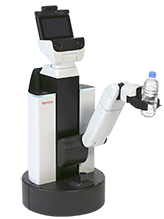
\includegraphics[width=0.25\textwidth]{images/toyota_hsr.png}
		\vspace{-10pt}
		\caption{Toyota HSR}
		\label{fig:toyotaHSR}
	\end{center}

	\vspace{-25pt}
	\begin{center}
		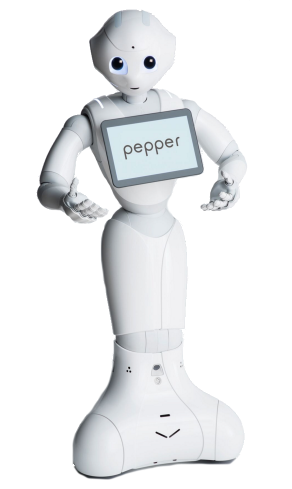
\includegraphics[width=0.20\textwidth]{images/softbank_pepper.png}
		\vspace{-10pt}
		\caption{Softbank / Aldebaran Pepper}
		\label{fig:softbank-pepper}
	\end{center}
\end{wrapfigure}
Each league points out to a different aspect of service robotics, reason for which they target specific abilities.


\subsection{Domestic Standard Platform League}
The \iterm{Domestic Standard Platform League}(DSPL) has as main goal to assist humans in a domestic environment, paying special attention to elderly people and people suffering of illness or disability. In consequence, the DSPL focuses on Ambient Intelligence, Computer Vision, Object Manipulation, Safe Indoor Navigation and Mapping, and Task Planning.

The robot to be used in the DSPL is the Toyota HSR, shown in Figure 1.1.

\subsection{Social Standard Platform League}
With a 180 degree turn in Human Robot Interaction, the \iterm{Social Standard Platform League}(SSPL) takes robots away from the traditional passive servant role, for now the robot is the one who will actively look for interaction. From a party waiter in a home environment to a hostess in a museum or shopping mall, in \iterm{SSPL} look for the next user who may require its services. Hence, this league focuses on Human-Robot Interaction, Natural Language Processing, People Detection and Recognition, Reactive Behaviors, and Safe Outdoor Navigation and Mapping.

The robot to be used in the SSPL is the Softbank/Aldebaran Pepper, shown in Figure 1.2.

\subsection{Open Platform League}
The \iterm{Open Platform League}(OPL) has the same modus operandi used since the fundation of RoboCup@Home till 2017 when Standard Platform Leagues were created. With no hardware constrains, OPL is the league for teams who want to test their own robot designs and configuration, as well as for old at-homers. In this league robots are tested to their limits without having in mind design restriction, although the scope is similar to the DSPL. 


%% %%%%%%%%%%%%%%%%%%%%%%%%%%%%%%%%%%%%%%%%%%%%%%%%%%%%%%%%%%%%%%%%%%%%%%%%%%%
%%
%%    author(s): RoboCupAtHome Technical Committee(s)
%%  description: Introduction - Competition
%%
%% %%%%%%%%%%%%%%%%%%%%%%%%%%%%%%%%%%%%%%%%%%%%%%%%%%%%%%%%%%%%%%%%%%%%%%%%%%%
\section{Competition}
The competition consists of 2 \emph{Stages} and the \iterm{Finals}. Each stage consists of a series of \iterm{Tests} that are being held in a daily life environment. The best teams from \iterm{Stage~I} advance to \iterm{Stage~II} which consists of more difficult tests. The competition ends with the \emph{Finals} where only the two highest ranked teams of each sub-league compete to select the winner.

%% %%%%%%%%%%%%%%%%%%%%%%%%%%%%%%%%%%%%%%%%%%%%%%%%%%%%%%%%%%%%%%%%%%%%%%%%%%%
%%
%%    author(s): RoboCupAtHome Technical Committee(s)
%%  description: Introduction - Awards
%%
%% %%%%%%%%%%%%%%%%%%%%%%%%%%%%%%%%%%%%%%%%%%%%%%%%%%%%%%%%%%%%%%%%%%%%%%%%%%%
\section{Awards}
\label{sec:awards}
The RoboCup@Home league features the following \iterm{awards}.

\subsection{Winner of the competition}
For each league, there will be a 1st, 2nd, and 3rd place award.

%
% As of 2017, the Execs have decided to remove the Innovation Award since
% is rarely given and its discussion is time consuming.
%
% \subsection{Innovation award}
% \label{award:innovation}
% To honour outstanding technical and scientific achievements as well as applicable solutions in the @Home league, a special \iterm{innovation award} may be given to one of the participating teams. Special attention is being paid to making usable robot components and technology available to the @Home community.
% 
% The \iaterm{Executive Committee}{EC} members from the RoboCup@Home league nominate a set of candidates for the award. The \iaterm{Technical Committee}{TC} elects the winner. A TC member whose team is among the nominees is not allowed to vote.
% 
% There is no innovation award in case no outstanding innovation and no nominees, respectively.


%
% As of 2017, the TC have decided to add an award for the best alternate HRI method
% to bypass speech recognition.
%
\subsection{Best Human-Robot Interface award}
\label{award:hri}
To honour outstanding Human-Robot Interfaces developed for interacting with robots in the @Home league, a special \iterm{Best HR Interface award} may be given to one of the participating teams. Special attention is being paid to making the interface open and available to the @Home community.

The \iaterm{Executive Committee}{EC} members from the RoboCup@Home league nominate a set of candidates for the award. The \iaterm{Technical Committee}{TC} elects the winner. A TC member whose team is among the nominees is not allowed to vote.
 
There is no Best HR Interface award in case no outstanding interface and no nominees, respectively.

%
% As of 2013, the Execs have decided to remove the Innovation Award due to
% the lack of interest of the participants
%
% \subsection{Winner of the Technical Challenge}
% In parallel to the regular competition, the RoboCup@Home league features a \iterm{technical challenge}. The winner of the technical challenge is given a special \iterm{award for winning the technical challenge}.
%
% As with the innovation award, the award for winning the technical challenge is not given in case no team shows a \emph{sufficient performance}. The decision which team wins the technical challenge, and if the award is given at all, is conducted by the \iaterm{Technical Committee}{TC}.

\subsection{Skill Certificates}
  \label{award:skill}
  The @Home league features certificates for the robots best at a the skills below:
  \begin{itemize}
   \item Navigation
   \item Manipulation
   \item Speech Recognition
   \item Person Recognition
  \end{itemize}
  
  A team is given the certificate if it scored at least 75\% of the attainable points for that skill.
  This is counted over all challenges, so e.g. if the robot scores manipulation points during the navigation test to open the door, that will count for the Manipulation-certificate.
  The certificate will only be handed out if the team is \emph{not} the overall winner of the competition. 


% Local Variables:
% TeX-master: "Rulebook"
% End:
